\documentclass[11pt, a4paper]{article}
\usepackage{pdfpages}
\usepackage{parallel}
\usepackage[T2A]{fontenc}
\usepackage{ucs}
\usepackage[utf8x]{inputenc}
\usepackage[polish,english,russian]{babel}
\usepackage{hyperref}
\usepackage{rotating}
\usepackage[inner=2cm,top=1.8cm,outer=2cm,bottom=2.3cm,nohead]{geometry}
\usepackage{listings}
\usepackage{graphicx}
\usepackage{wrapfig}
\usepackage{longtable}
\usepackage{indentfirst}
\usepackage{array}
\usepackage{tikzsymbols}
\usepackage{soul}
\usepackage[ruled,vlined]{algorithm2e}
%\counterwithout{figure}{section} 

\usepackage{url}
\makeatletter
\g@addto@macro{\UrlBreaks}{\UrlOrds}
\makeatother

\newcolumntype{P}[1]{>{\raggedright\arraybackslash}p{#1}}
\frenchspacing
\usepackage{fixltx2e} %text sub- and superscripts
\usepackage{icomma} % коскі ў матэматычным рэжыме
\PreloadUnicodePage{4}

\newcommand{\longpage}{\enlargethispage{\baselineskip}}
\newcommand{\shortpage}{\enlargethispage{-\baselineskip}}

\def\switchlang#1{\expandafter\csname switchlang#1\endcsname}
\def\switchlangbe{
\let\saverefname=\refname%
\def\refname{Літаратура}%
\def\figurename{Іл.}%
}
\def\switchlangen{
\let\saverefname=\refname%
\def\refname{References}%
\def\figurename{Fig.}%
}
\def\switchlangru{
\let\saverefname=\refname%
\let\savefigurename=\figurename%
\def\refname{Литература}%
\def\figurename{Рис.}%
}

\hyphenation{admi-ni-stra-tive}
\hyphenation{ex-pe-ri-ence}
\hyphenation{fle-xi-bi-li-ty}
\hyphenation{Py-thon}
\hyphenation{ma-the-ma-ti-cal}
\hyphenation{re-ported}
\hyphenation{imp-le-menta-tions}
\hyphenation{pro-vides}
\hyphenation{en-gi-neering}
\hyphenation{com-pa-ti-bi-li-ty}
\hyphenation{im-pos-sible}
\hyphenation{desk-top}
\hyphenation{elec-tro-nic}
\hyphenation{com-pa-ny}
\hyphenation{de-ve-lop-ment}
\hyphenation{de-ve-loping}
\hyphenation{de-ve-lop}
\hyphenation{da-ta-ba-se}
\hyphenation{plat-forms}
\hyphenation{or-ga-ni-za-tion}
\hyphenation{pro-gramming}
\hyphenation{in-stru-ments}
\hyphenation{Li-nux}
\hyphenation{sour-ce}
\hyphenation{en-vi-ron-ment}
\hyphenation{Te-le-pathy}
\hyphenation{Li-nux-ov-ka}
\hyphenation{Open-BSD}
\hyphenation{Free-BSD}
\hyphenation{men-ti-on-ed}
\hyphenation{app-li-ca-tion}

\def\progref!#1!{\texttt{#1}}
\renewcommand{\arraystretch}{2} %Іначай формулы ў матрыцы зліпаюцца з лініямі
\usepackage{array}

\def\interview #1 (#2), #3, #4, #5\par{

\section[#1, #3, #4]{#1 -- #3, #4}
\def\qname{LVEE}
\def\aname{#1}
\def\q ##1\par{{\noindent \bf \qname: ##1 }\par}
\def\a{{\noindent \bf \aname: } \def\qname{L}\def\aname{#2}}
}

\def\interview* #1 (#2), #3, #4, #5\par{

\section*{#1\\{\small\rm #3, #4. #5}}
\ifx\ParallelWhichBox\undefined%
    \addcontentsline{toc}{section}{#1, #3, #4}%
\else%
\ifnum\ParallelWhichBox=0%
    \addcontentsline{toc}{section}{#1, #3, #4}%
\fi\fi%

\def\qname{LVEE}
\def\aname{#1}
\def\q ##1\par{{\noindent \bf \qname: ##1 }\par}
\def\a{{\noindent \bf \aname: } \def\qname{L}\def\aname{#2}}
}

\newcommand{\interviewfooter}[1]{
\vskip 1em
\noindent \textit{#1}
}

\switchlang{ru}
\begin{document}

\title{1993 "--- Evergreen Diamond XL trackball}
\date{}
\maketitle
\selectlanguage{russian}
Трекбол Diamond XL выпущен калифорнийской компанией Evergreen Systems International, основанной в 1980 году и специализировавшейся на высококачественных трекболах для промышленного и военного применения.

Разработчик позиционировал трекболы Diamond как замену мыши в компьютерных системах, где требуются быстрые и точные функции наведения (CAD/CAM, графика, рабочие станции, киоски и т.д.), а также в промышленных и военных системах, где мышь не подходит для использования из-за нехватки места, суровых условий эксплуатации, среды или других факторов.

Первые упоминания данной модели в рекламных материалах датируются 1993 годом \cite{nasa}.

\begin{figure}[h]
    \centering
    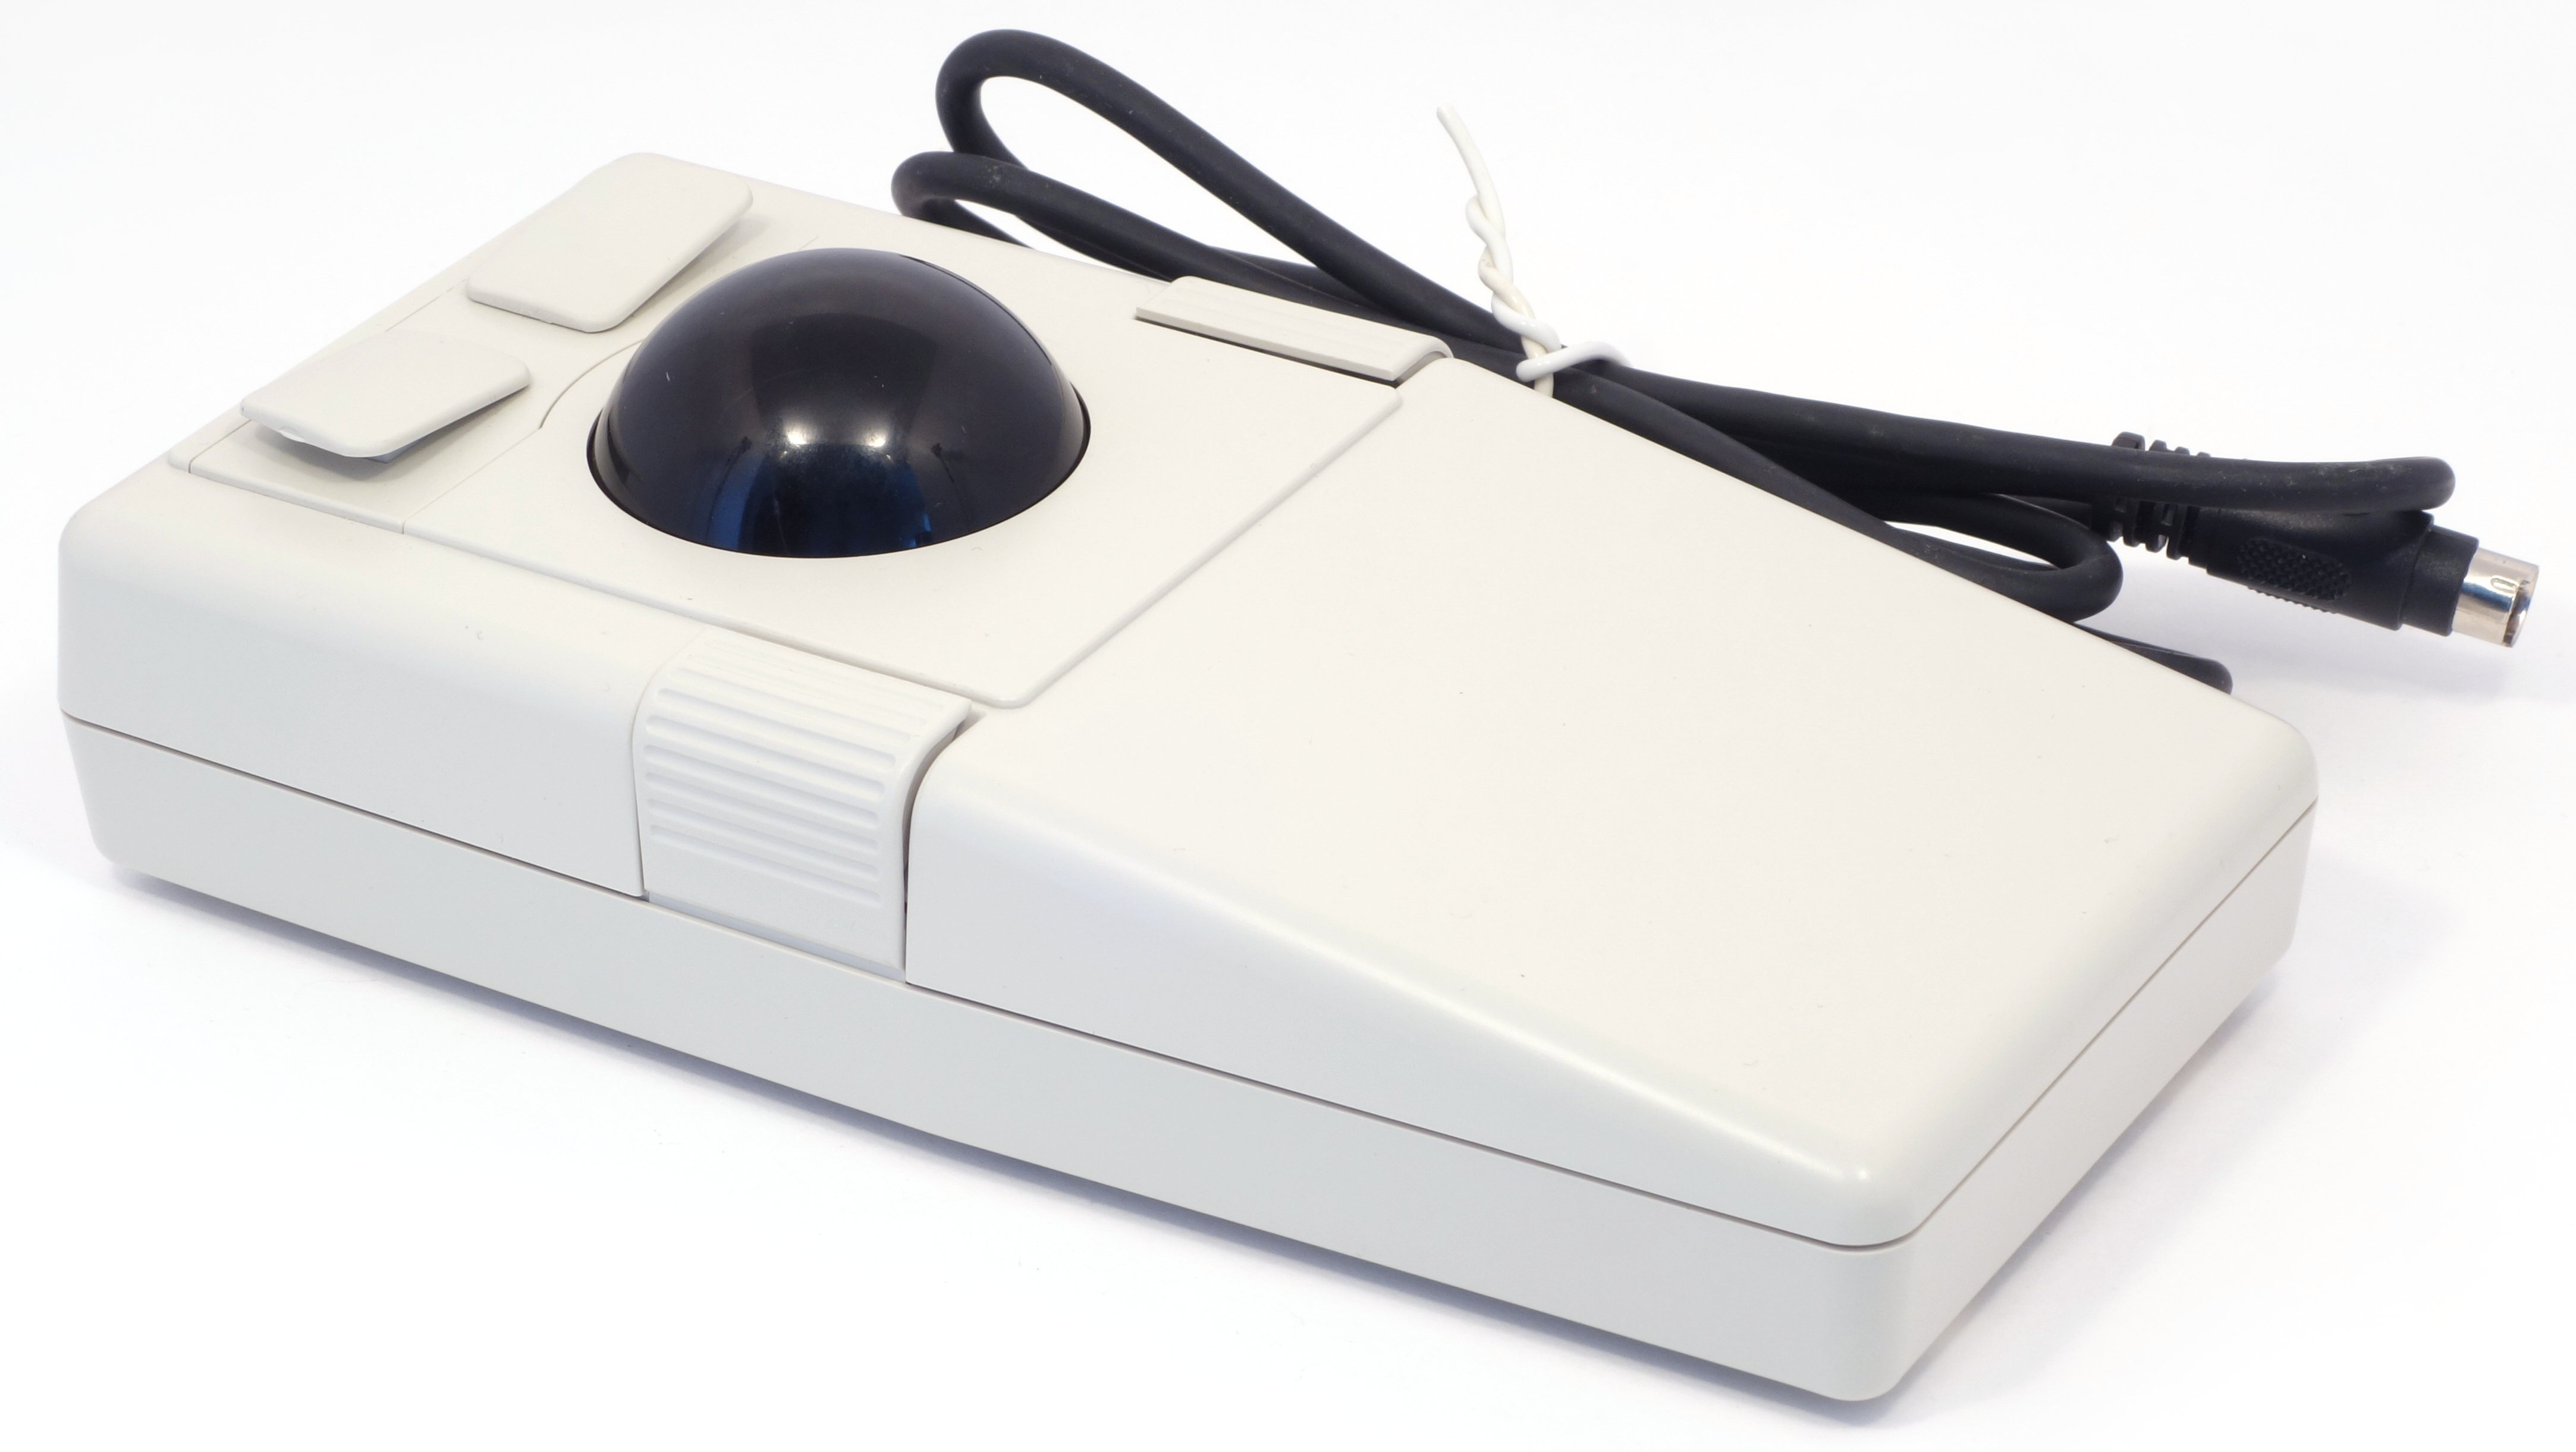
\includegraphics[scale=0.3]{1993_evergreen_diamond_xl_trackball/pic_30.jpg}
    \caption{Трекбол Diamond XL}
    \label{fig:DiamondXL}
\end{figure}

На рис. \ref{fig:DiamondXLTopBottom} можно видеть верхнюю и нижнюю стороны трекбола.
На верхней части корпуса отсутствуют какие-либо надписи; корпус имеет гладкую матовую поверхность и ребристые боковые клавиши для их более легкой тактильной идентификации. На нижней части корпуса присутствуют резиновые ножки, обеспечивающие надежную фиксацию на поверхности стола, маркировка производителя и модели.

\begin{figure}[h]
    \centering
    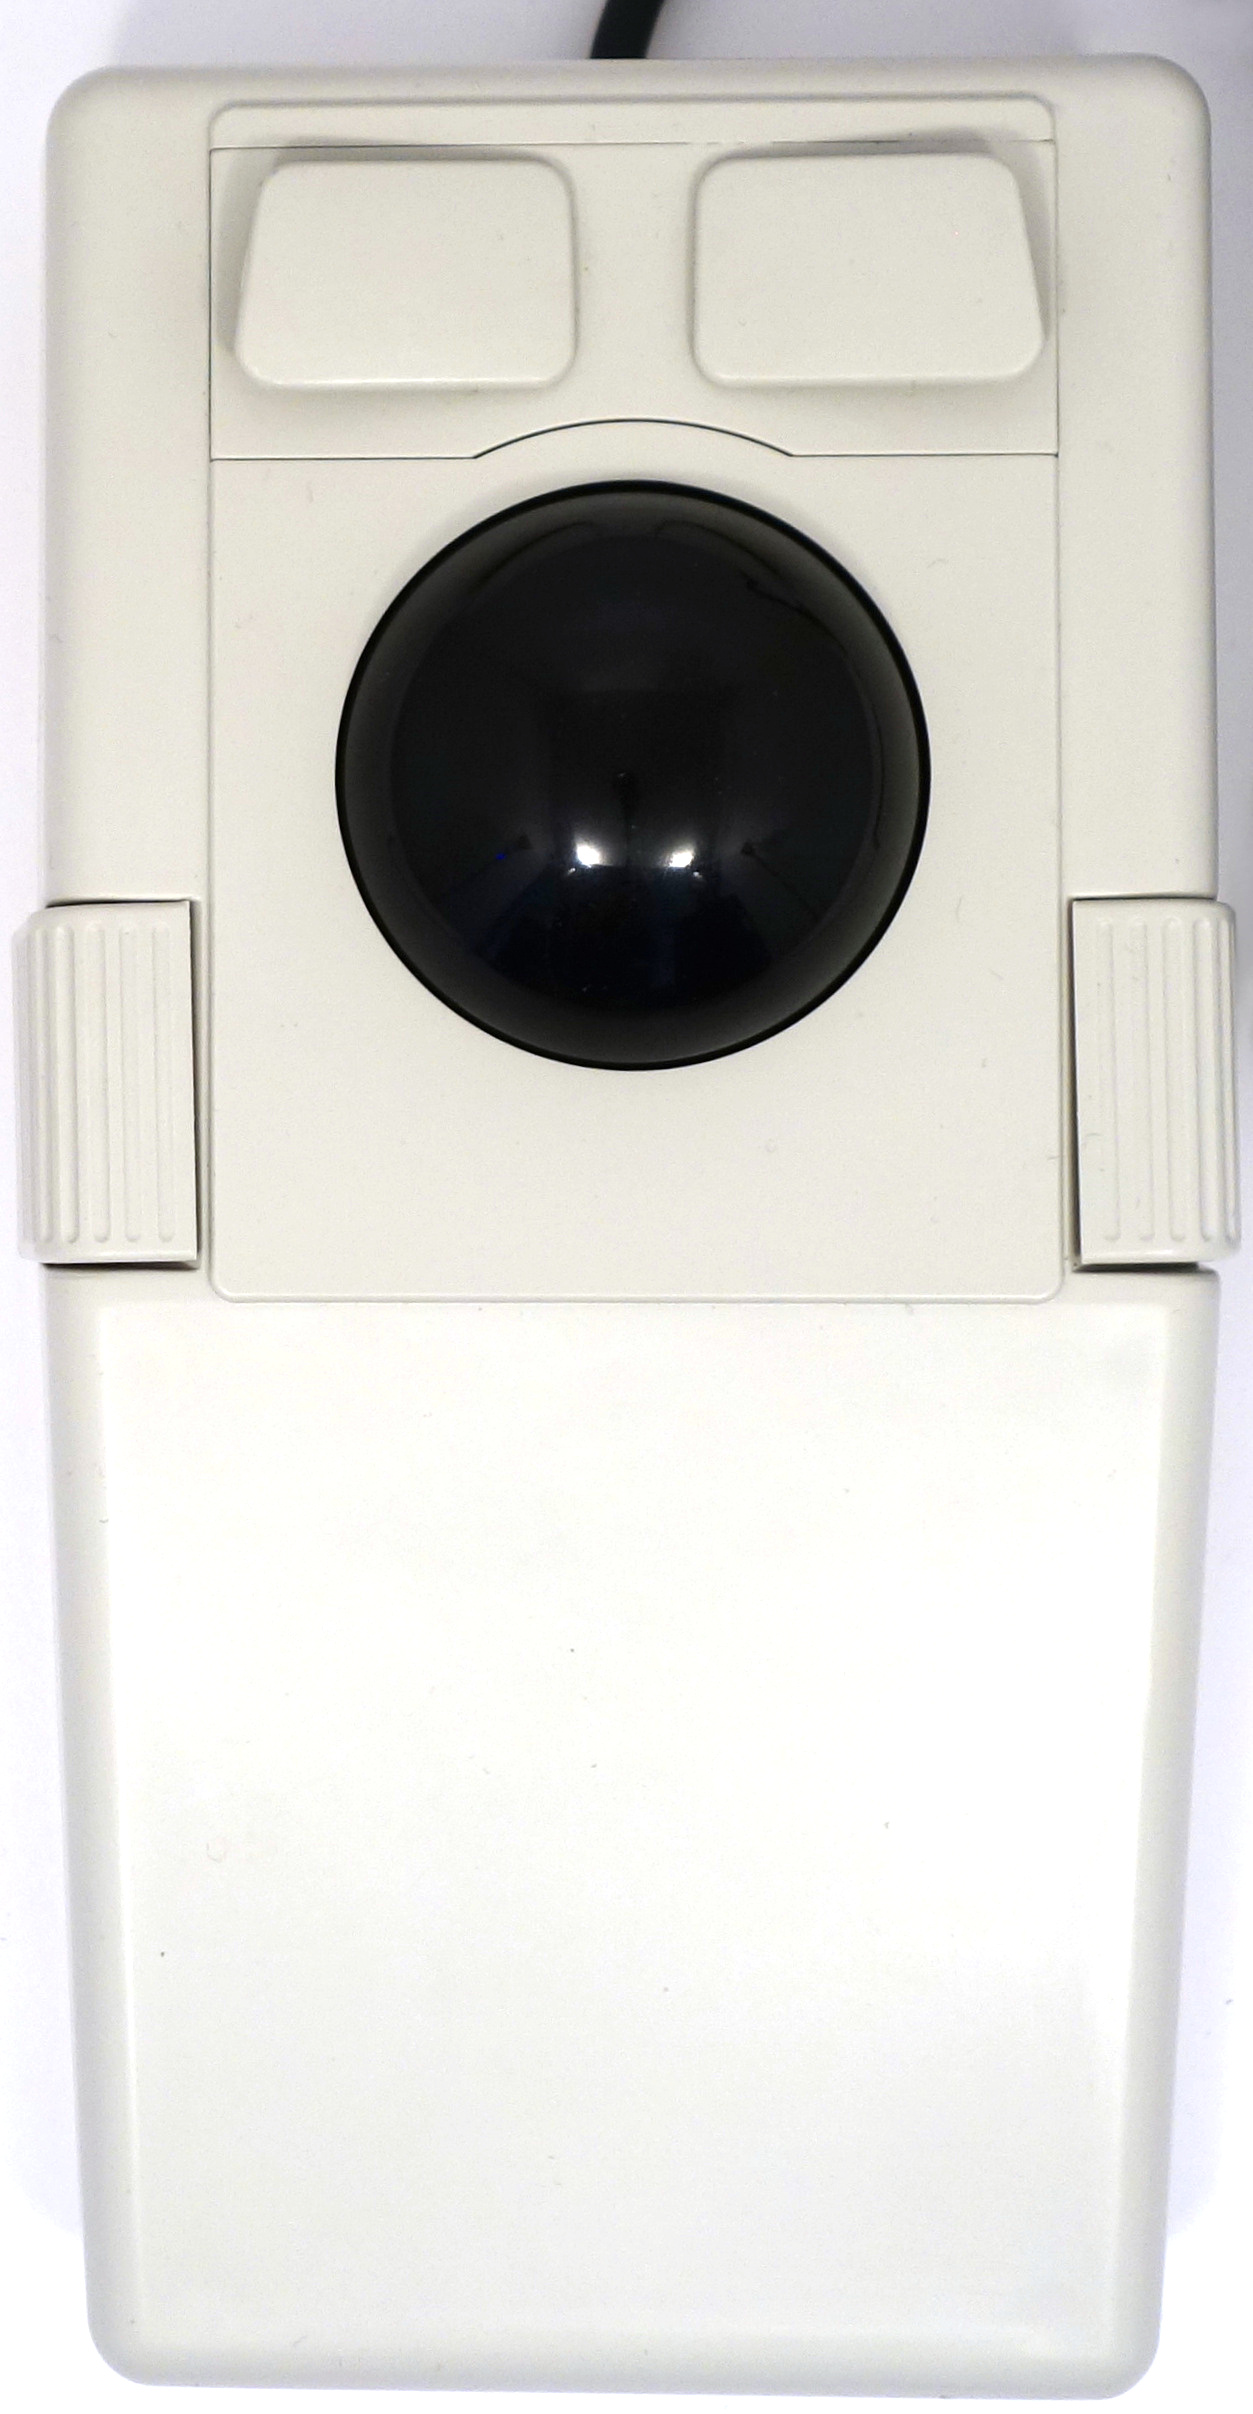
\includegraphics[scale=0.35]{1993_evergreen_diamond_xl_trackball/top_30.jpg}
    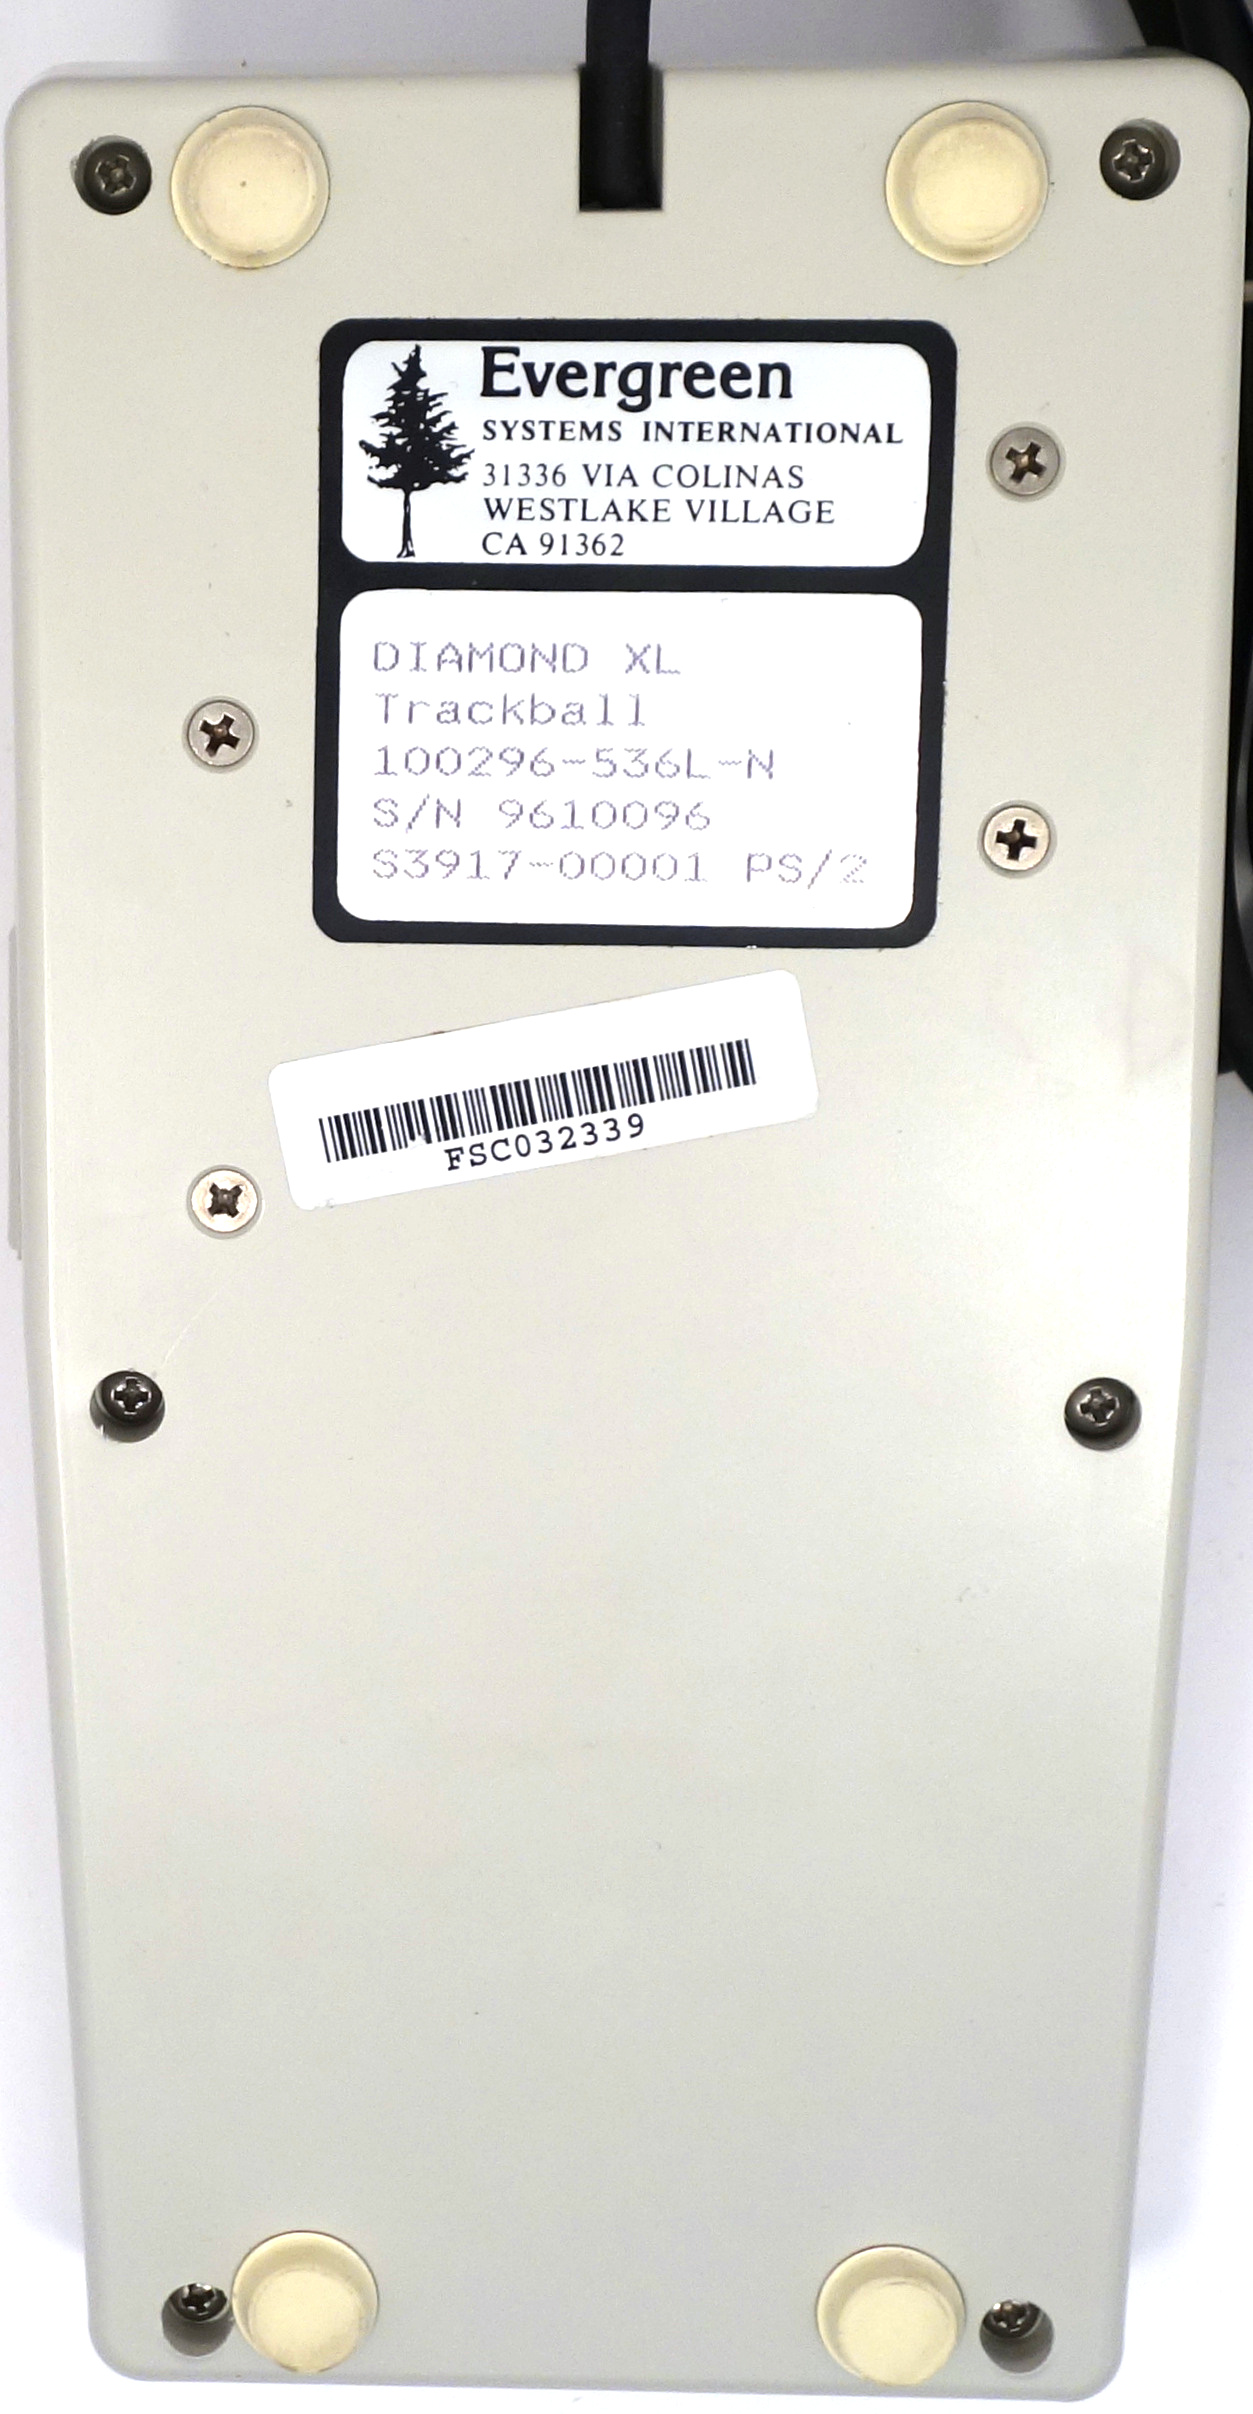
\includegraphics[scale=0.35]{1993_evergreen_diamond_xl_trackball/bottom_30.jpg}
    \caption{Diamond XL, вид сверху и снизу}
     \label{fig:DiamondXLTopBottom}
\end{figure}

Данное устройство является весьма габаритным (рис. \ref{fig:DiamondXLSize}). Диаметр шара составляет 51 мм (2 дюйма).

\begin{figure}[h]
    \centering
    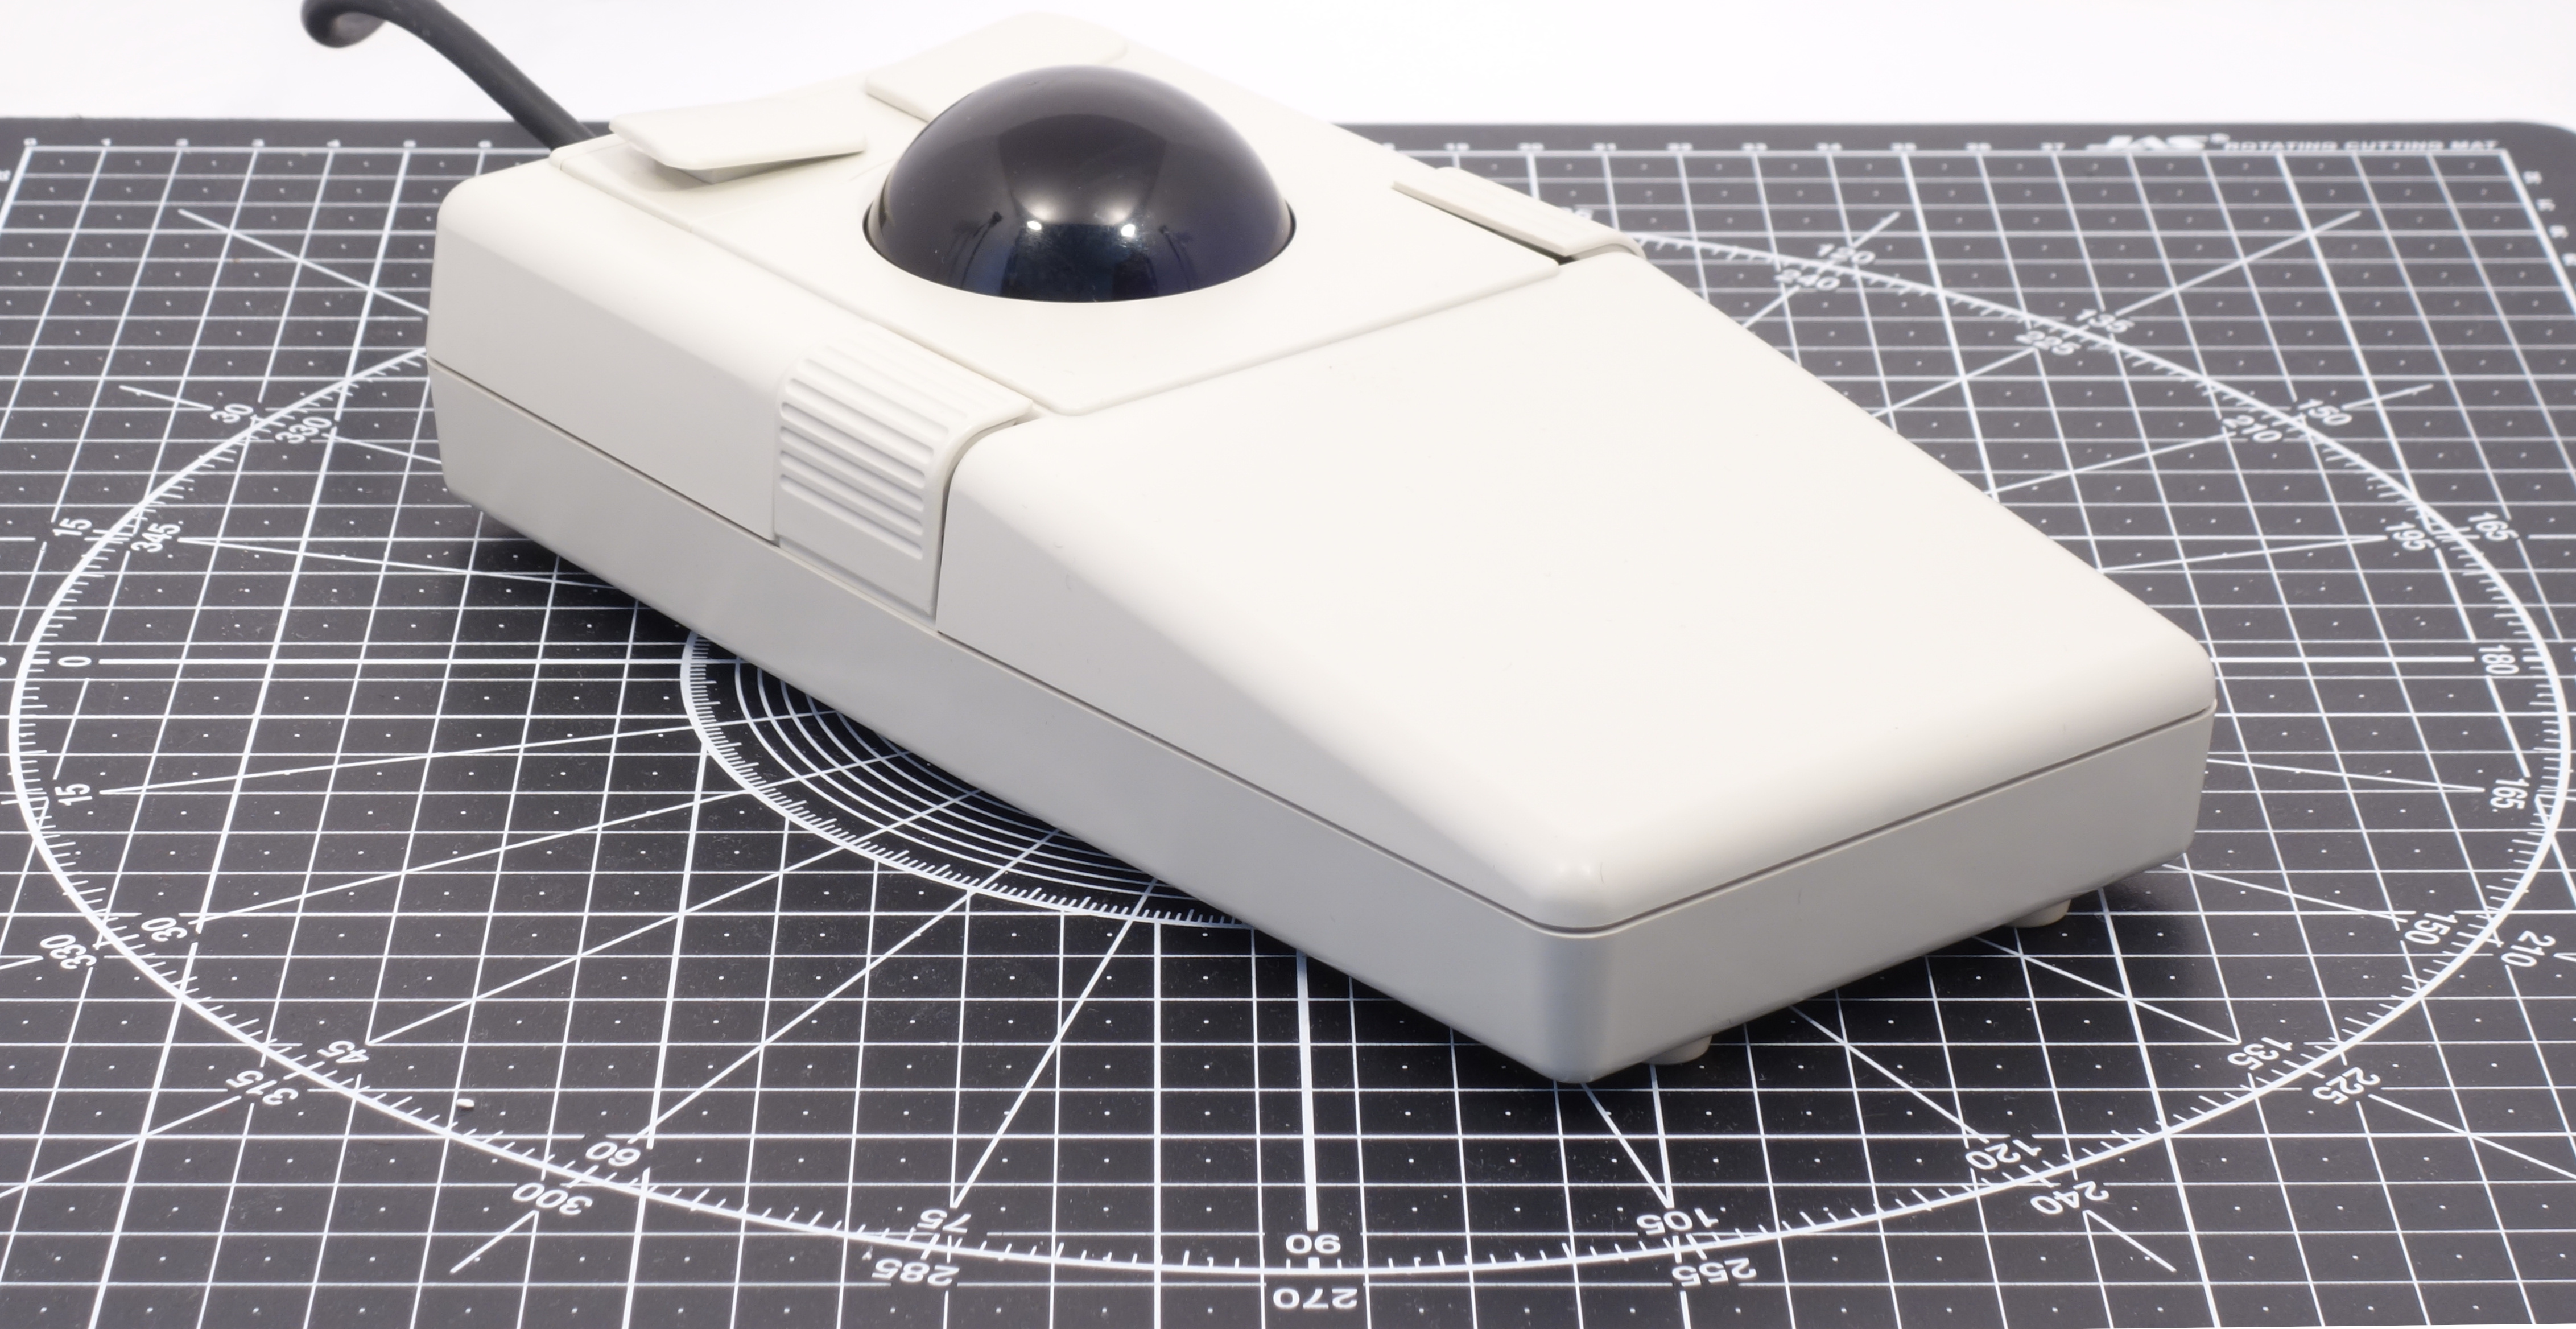
\includegraphics[scale=0.35]{1993_evergreen_diamond_xl_trackball/size.jpg}
    \caption{Изображение Diamond XL на размерном коврике с шагом сетки 1~см}
    \label{fig:DiamondXLSize}
\end{figure}

Трекбол симметричен и одинаково удобен при использовании как правой так и левой рукой. Основная (левая) кнопка мыши расположена под большим пальцем для удобства выбора и перетаскивания объектов (рис. \ref{fig:DiamondXLHand}), при этом остальные пальцы остаются свободными для позиционирования курсора. Роль средней кнопки играет пара наклонных клавиш, расположенных за шаром (в данной версии трекбола они имеют наклон к центру, а в упоминавшейся на сайте производителя пятикнопочной версии \cite{evergreen} за шаром расположен блок из трех таких клавиш, повернутых на 90 градусов и имеющих наклон к краю корпуса). Правая кнопка симметрична левой и нажимается мизинцем. В некоторых модификациях правостороннее или левостороннее управление выбирается с помощью переключателей конфигурации, расположенных в вырезе в нижней части корпуса, однако в данном экземпляре оно реализуется лишь на уровне драйвера.

Трекбол выпускался в модификациях c различными интерфейсами, что позволяло использовать их с компьютерами SUN, DEC, Hewlett Packard (шина HP/HIL), IBM, SGI и Macintosh с шиной USB. В частности, трекбол DTXL3 с шиной HP/HIL производился по лицензии Hewlett Packard, и позиционировался как прямая замена мыши HP/HIL, а также снятого с производства собственного трекбола Hewlett Packard HP M1309A \cite{dtxl3, hphil}. Следы такой ориентации Diamond XL можно заметить в дизайне корпуса: дальняя от пользователя стенка включает две технологические площадки, предназначенные для установки гнезд подключения к шине HP/HIL (рис. \ref{fig:DiamondXLHand}).

\begin{figure}[h]
    \centering
    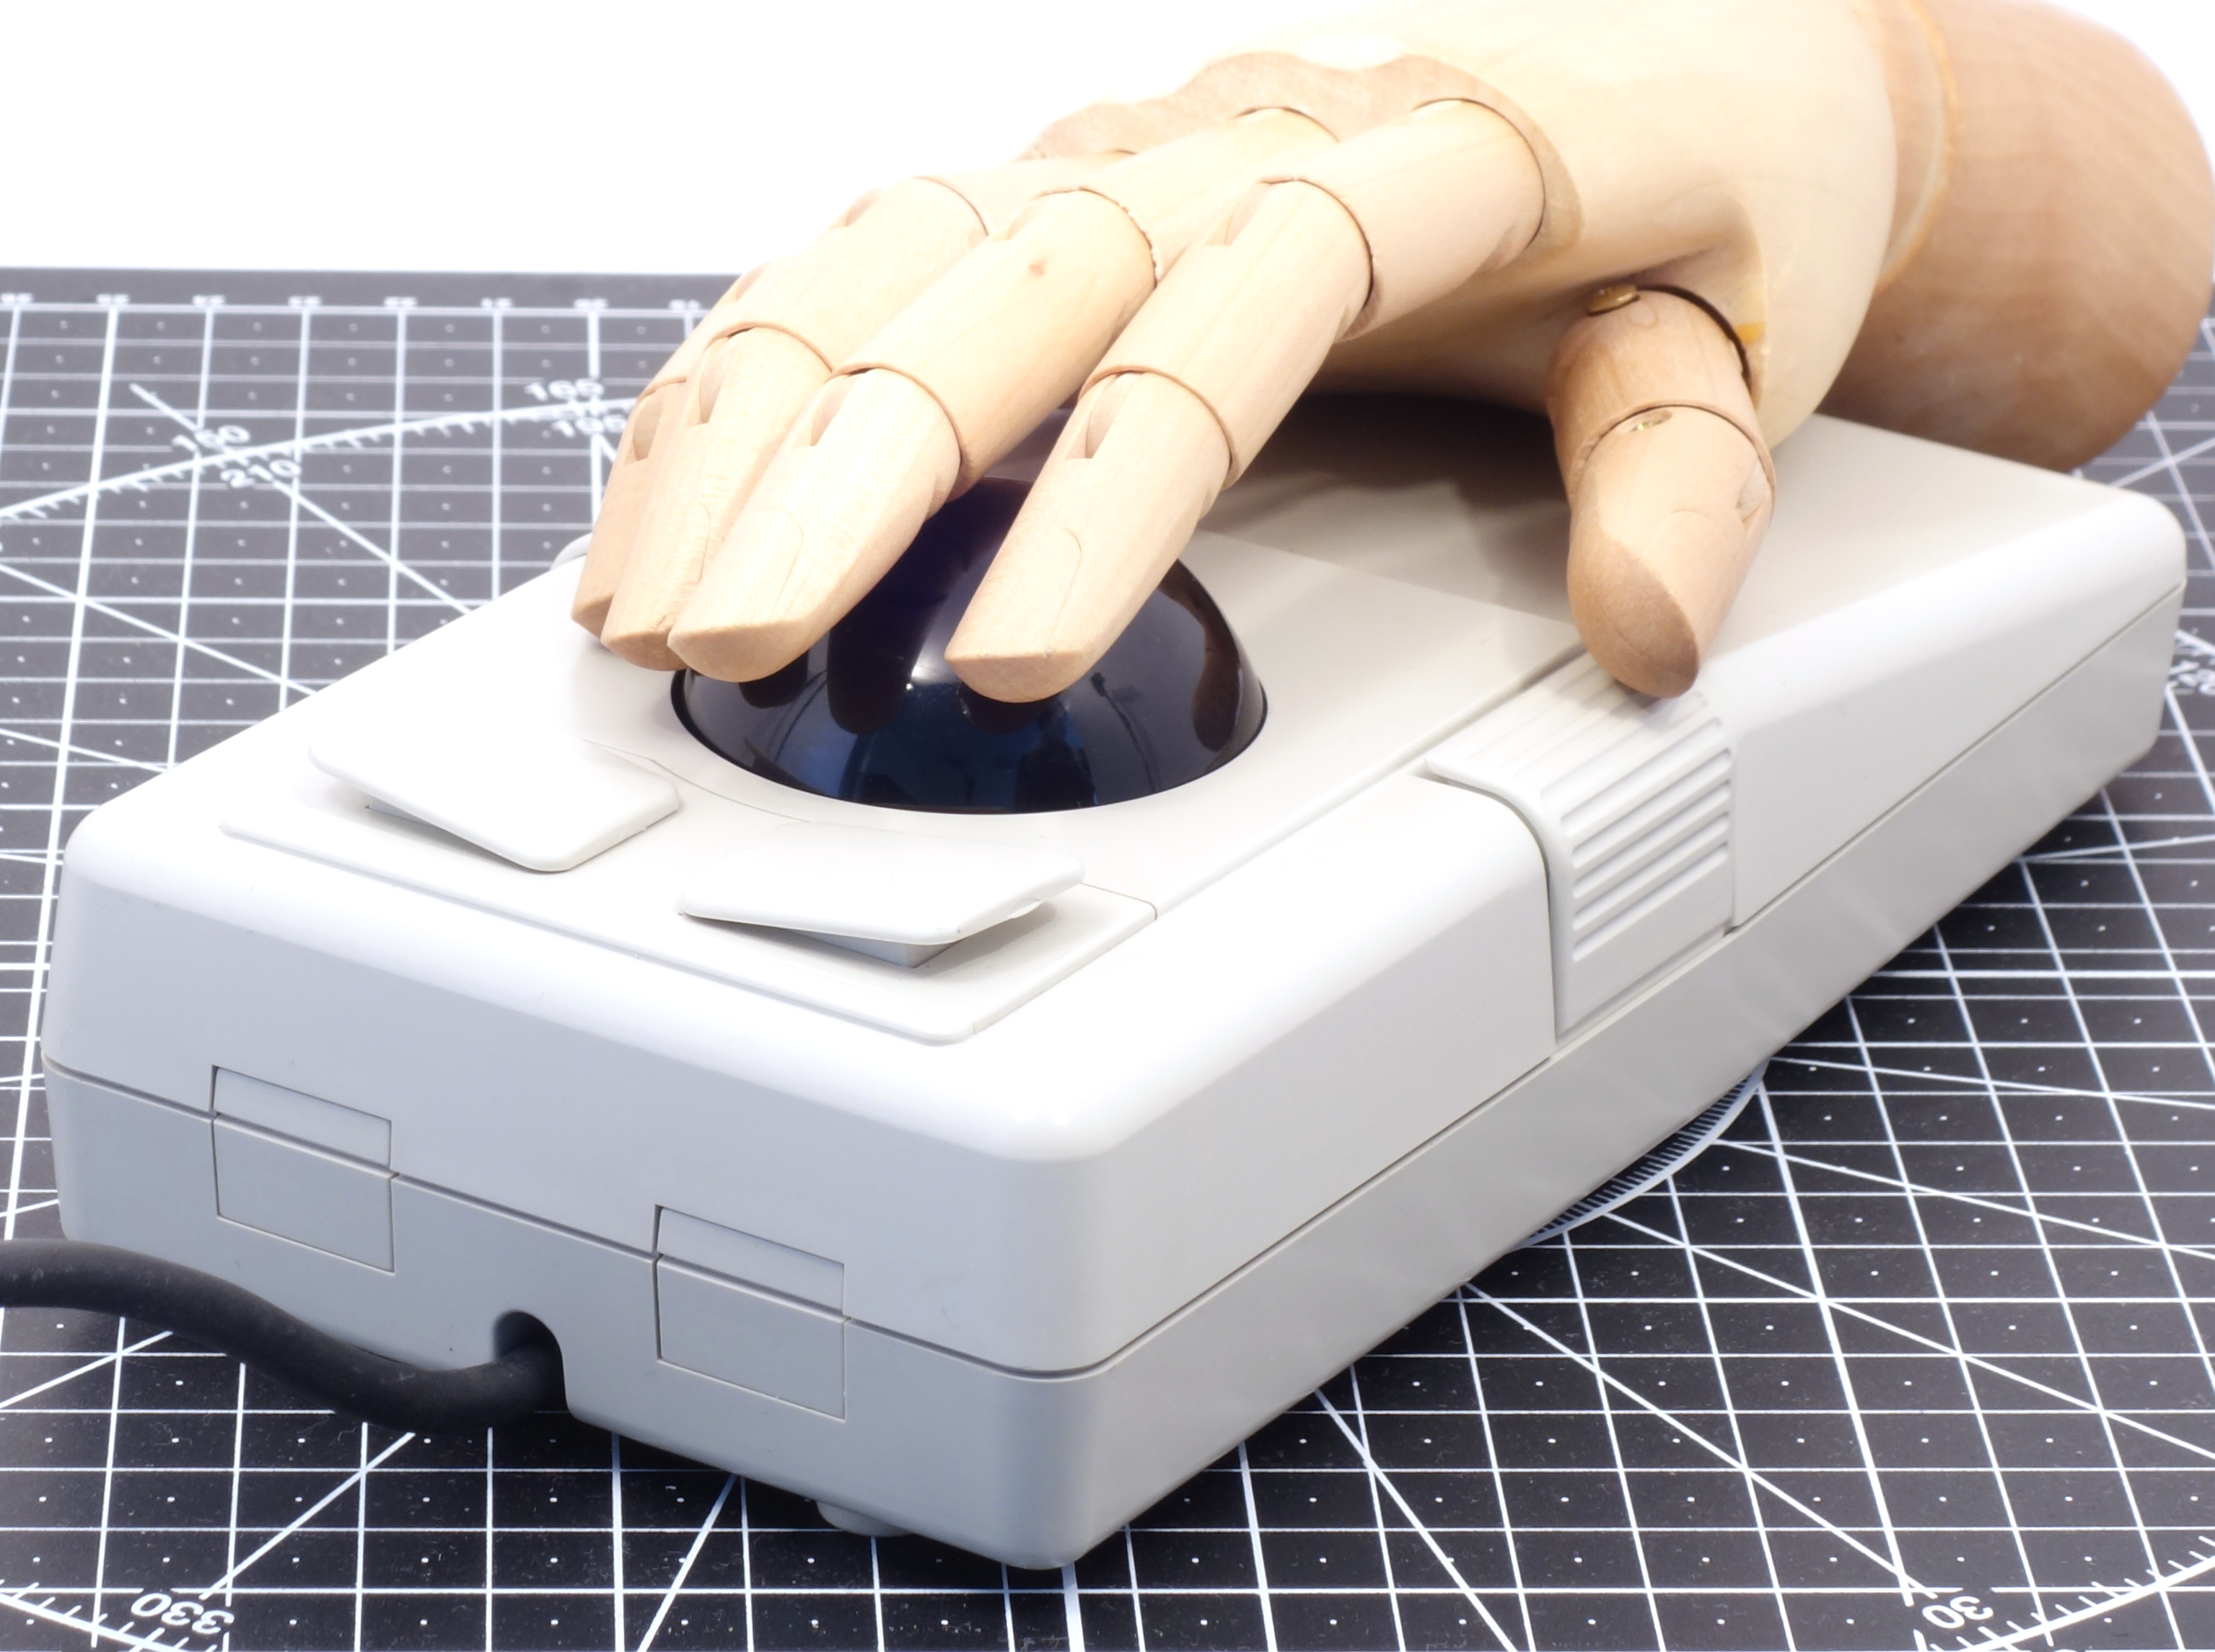
\includegraphics[scale=0.4]{1993_evergreen_diamond_xl_trackball/hand_30.jpg}
    \caption{Diamond XL с моделью руки человека}
    \label{fig:DiamondXLHand}
\end{figure}

Внутреннее устройство данного трекбола показано на рис. \ref{fig:DiamondXLInside}. Как можно видеть,  трекбол выполнен по традиционной оптомеханической схеме. Также следует отметить, что ролики реализованы с использованием подшипников и металлических осей, предназначенных для того, чтобы обеспечить максимальную надежность и долговечность конструкции. На это делается упор и в описании производителя, где среди особенностей устройства подчеркивается полностью металлические механические части, валы повышенной твердости из азотированной стали с прецизионными шарикоподшипниками и переключатели с позолоченными пружинными контактами \cite{dtxl3}.

Извлечение шара для чистки трекбола невозможно без разборки корпуса.

\begin{figure}[h]
    \centering
    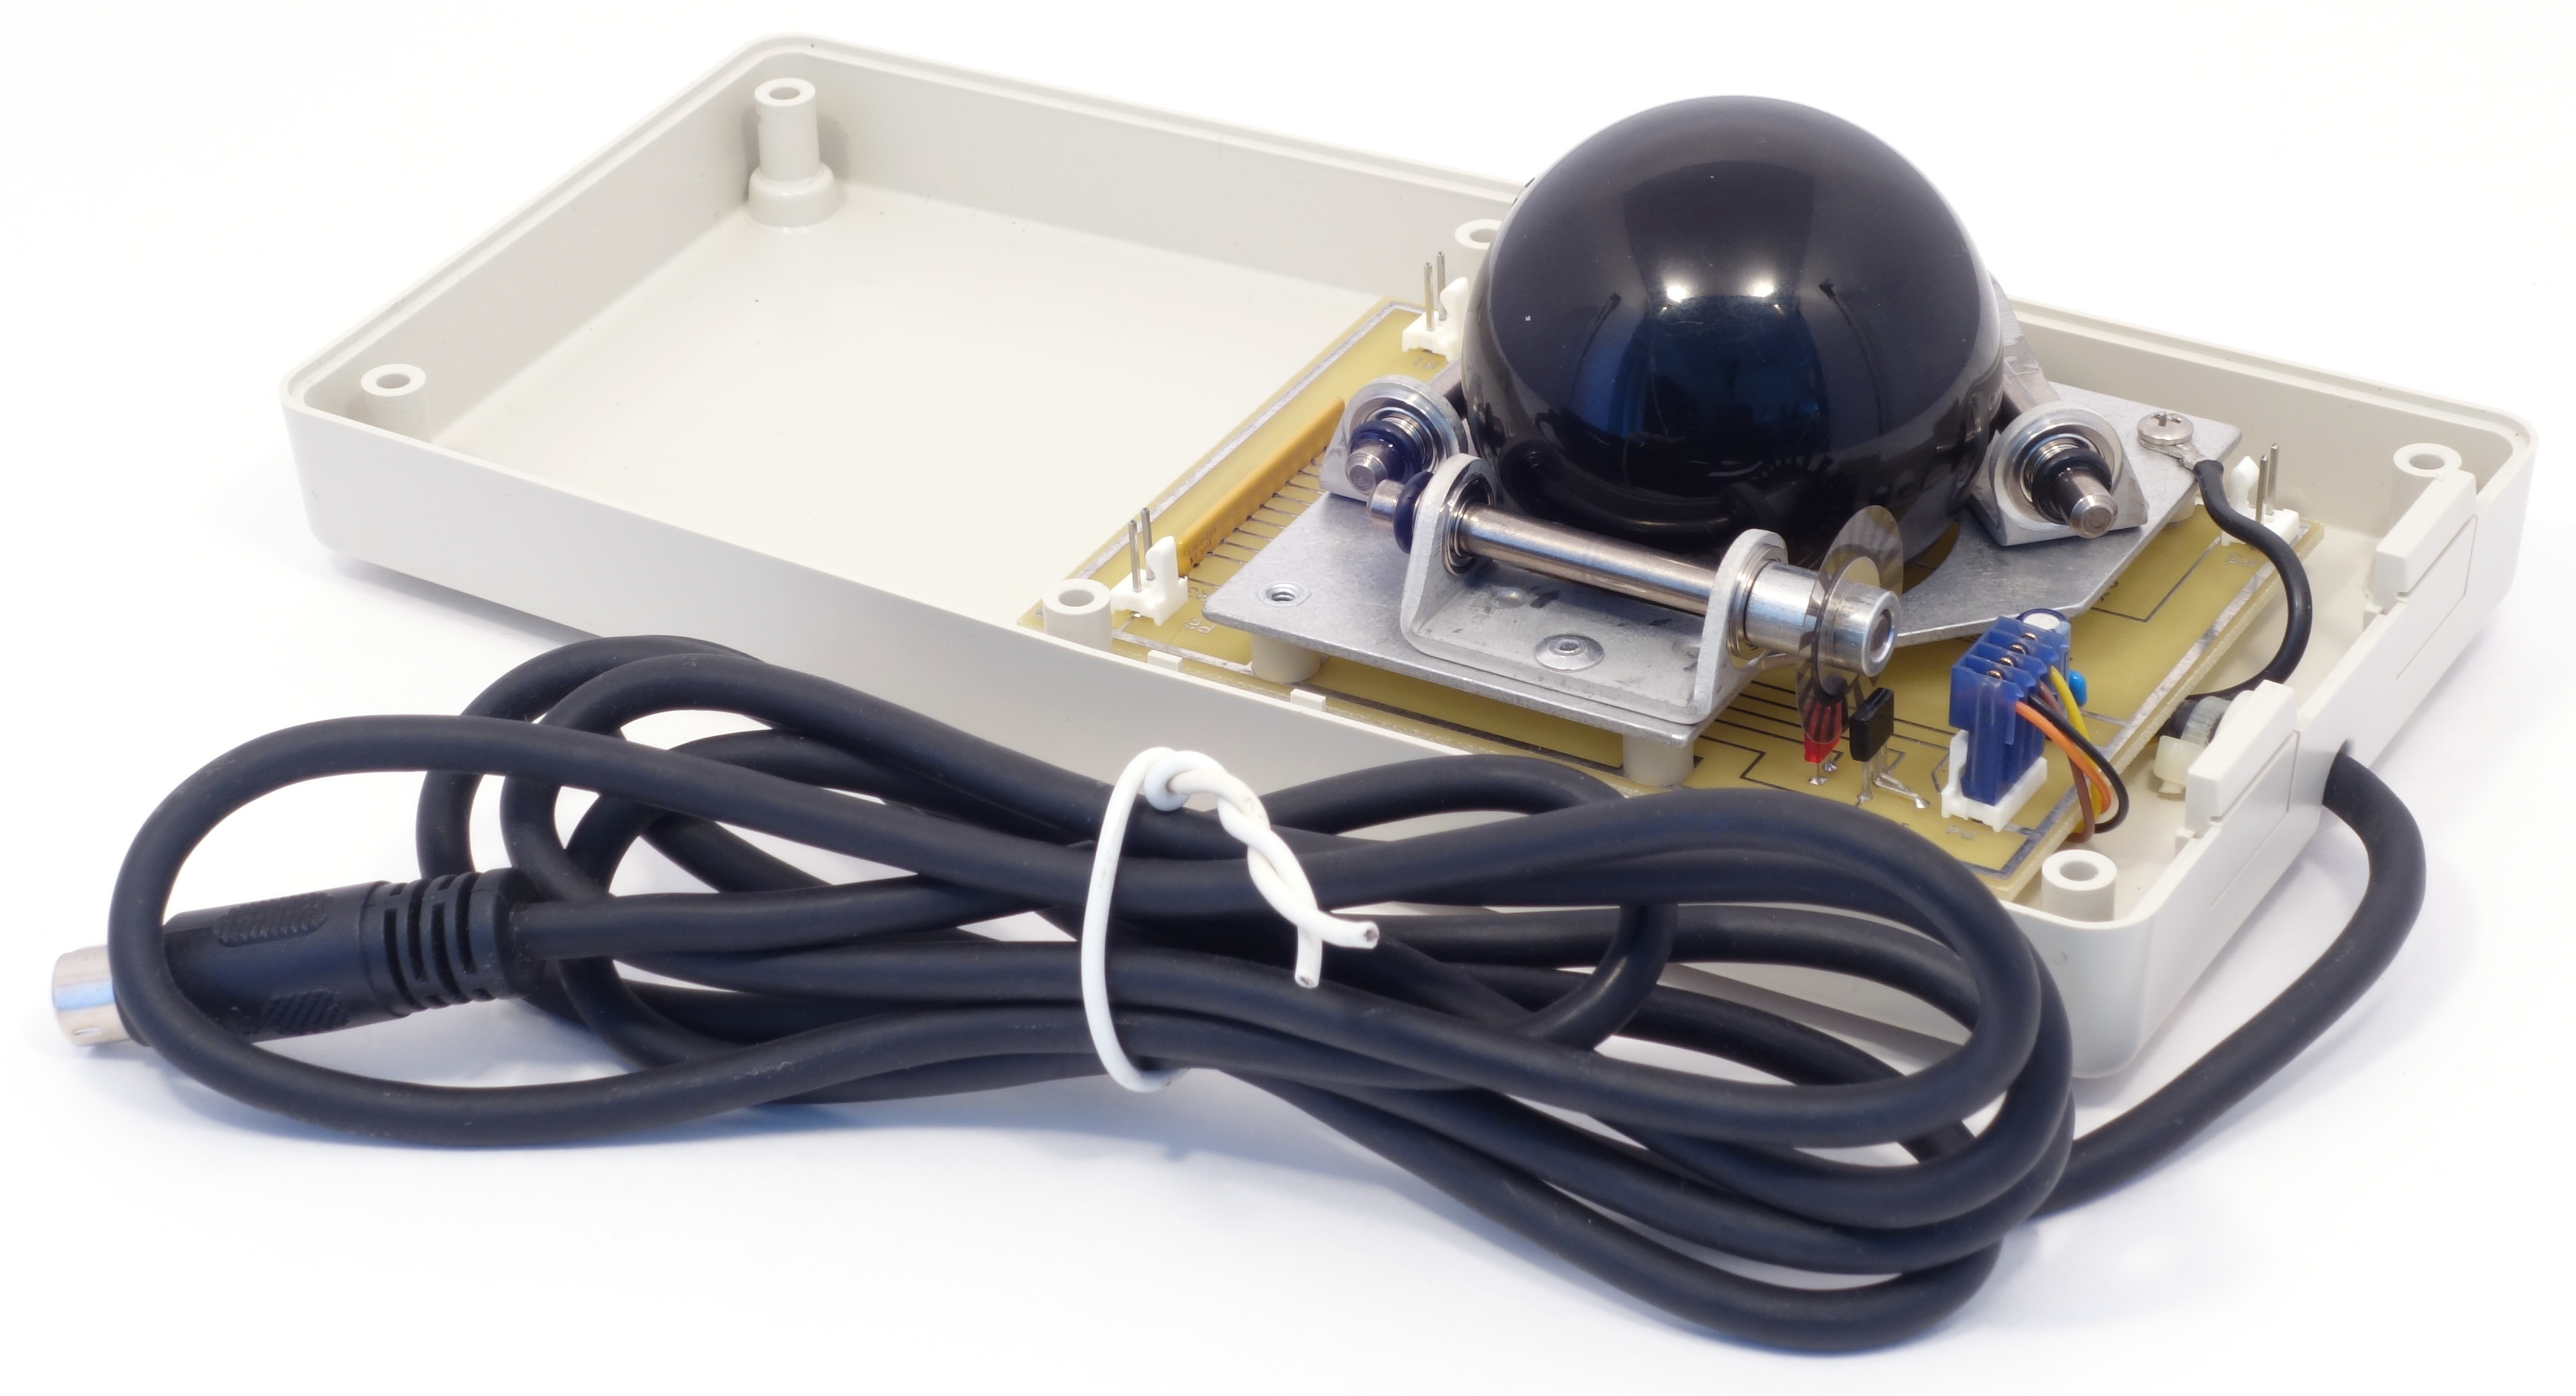
\includegraphics[scale=0.4]{1993_evergreen_diamond_xl_trackball/inside_30.jpg}
    \caption{Diamond XL в разобранном состоянии}
    \label{fig:DiamondXLInside}
\end{figure}

\begin{thebibliography}{9}
\bibitem{evergreen} Evergreen Systems International home page. \url{https://web.archive.org/web/19970102174426/http://trackballs.com:80/}
\bibitem{dtxl3} Keyton Computer -- Trackball \url{http://keyton.co.jp/products/UEVE/DTXL3.html}
\bibitem{hphil} Diamond XL HP-HIL trackball \url{https://web.archive.org/web/19970328230321/http://www.trackballs.com/xlhil.htm}
\bibitem{nasa} NASA Tech Briefs, November 1993. Volume 17, No. 11. -- p. 60 \url{https://archive.org/details/NASA_NTRS_Archive_20100030364/page/n59/mode/2up}
\end{thebibliography}
\end{document}
